\chapter{The Proposed Solution}\pagestyle{fancy}\setlength{\parindent}{3em}
\label{chap:proposed-solution}

The solution is an image processing pipeline that would extract from the side picture of a tire the markings written on it. These are present in the form of embossed letters on the tire's exterior walls. By desiring to not have a complex setup and not require supplementary light sources, the system was tested on images taken only with ambient light. This proved to increase the problem's difficulty quite considerably when it came to detecting the regions of text, because the contrast between the embossed letters and the background image got even smaller. Multiple approaches were considered in section \ref{sec:text-detection} Text Detection and in the end one proved fruitful in delivering acceptable results.

The system's stages are described in the following sections:

%%%%%%%%%%%%%%%%%%%%%%%%%%%%%%%%%%%%%%%%%%%%%%%%%%%%%%%%%%%%%%%%%%%%%%%%%%%%%%%%%%%%%%%%%%%%%%%%%%%%%%%%%%%%%%%%%%%%%%%%
%%%%%%%%%%%%%%%%%%%%%%%%%%%%%%%%%%%%%%%%%%%%%%%%%%%%%%%%%%%%%%%%%%%%%%%%%%%%%%%%%%%%%%%%%%%%%%%%%%%%%%%%%%%%%%%%%%%%%%%%
%%%%%%%%%%%%%%%%%%%%%%%%%%%%%%%%%%%%%%%%%%%%%%%%%%%%%%%%%%%%%%%%%%%%%%%%%%%%%%%%%%%%%%%%%%%%%%%%%%%%%%%%%%%%%%%%%%%%%%%%
\section{Tire Unwrapping (Stage 1)}\label{sec:tire-unwrapping}

As a first stage, I wanted to extract only the tire from the input image. This would help because the information I am interested in is located on it. I would also like to unwrap the tire from its disk shape (a circle with a smaller circle as a hole inside of it) into a rectangular one in order to have the writing from left to right rather than in all directions like if it was in a circle.

To better explain how this was accomplished, this stage was split in multiple steps:

%%%%%%%%%%%%%%%%%%%%%%%%%%%%%%%%%%%%%%%%%%%%%%%%%%%%%%%%%%%%%%%%%%%%%%%%%%%%%%%%%%%%%%%%%%%%%%%%%%%%%%%%%%%%%%%%%%%%%%%%
\subsection{Circle Detection}

I detect where in the image are the circles representing the outer and inner borders of the tire and get their center's coordinates. The two detected circles might not have a common center because of the imperfections in taking the images, but I account and try to correct for that through a series of heuristics.

Because this is the beginning of the pipeline, I introduced a step to \hyperref[subsubsec:equalization]{equalization} the images and have some independence from the lighting conditions. Then I detected the first circles in the image using \hyperref[subsubsec:hough_circles_transform]{Hough Circle Transform} and filtered its output through a series of \hyperref[subsubsec:circ_det_heuristics]{heuristics}.

%%%%%%%%%%%%%%%%%%%%%%%%%%%%%%%%%%%%%%%%%%%%%%%%%%%%%%%%%%%%
%%% a) EQUALIZATION                                      %%%
%%%%%%%%%%%%%%%%%%%%%%%%%%%%%%%%%%%%%%%%%%%%%%%%%%%%%%%%%%%%
\subsubsection{Equalization}
\label{subsubsec:equalization}

\paragraph*{Accomplishes:}\mbox{}\par
Lighting conditions are not controlled and this might result in low contrast in some areas of the image. Here we ensure a constant contrast across the entire image and that the entire histogram is used. This increases the robustness of the overall system.

\paragraph*{Reasoning:}\mbox{}\par
The pixel in a black and white image is a representation of how bright that particular part of the image should be (0 is for no light and 255 is for maximum brightness on a 8 bit sensor). If we take a photo in broad daylight, the values of all the pixels could all be over 200 lets say. The image would appear as being washed-out and lacking details like Figure \ref{fig:tire_unwrapping-equalization-effect}a and would have a histogram looking like Figure \ref{fig:tire_unwrapping-hist_of_equalization_effect_a}. If the photo is taken in a dark environment and all pixel values are under 100, the image appears again quite dark and lacking detail, this is the case for Figure \ref{fig:tire_unwrapping-equalization-effect}b whose histogram is drawn in Figure \ref{fig:tire_unwrapping-hist_of_equalization_effect_b}. A solution is to use the space that remained unused in pixel values and stretch the existing pixel values to also cover those, thus increasing the contrast of the image and its level of detail. This action is called equalization and can be used to enhance the contrast in an image, like can be seen in Figure \ref{fig:tire_unwrapping-equalization-effect}c. Furthermore, it spreads the pixel values across their entire value range so that a under-light and an over-light picture's histogram would look similar (Figure \ref{fig:tire_unwrapping-hist_of_equalization_effect_c}). The histogram is a plot that has on the $X$ axis all possible pixel values and on the $Y$ axis the number of times that value appears in an image and usually is on a logarithmic scale.

\begin{figure}
    \centering
    \begin{minipage}[c]{0.5\linewidth}
        \includegraphics[width=7.95cm, keepaspectratio]{img/algos/tire_unwrapping-histogram_effect.jpg}
        \caption{Equalization demonstration: a) overexposed image, b) underexposed image, c) equalized image}
        \label{fig:tire_unwrapping-equalization-effect}
    \end{minipage}\hfill
    \begin{minipage}[c]{0.5\linewidth}
        \centering
        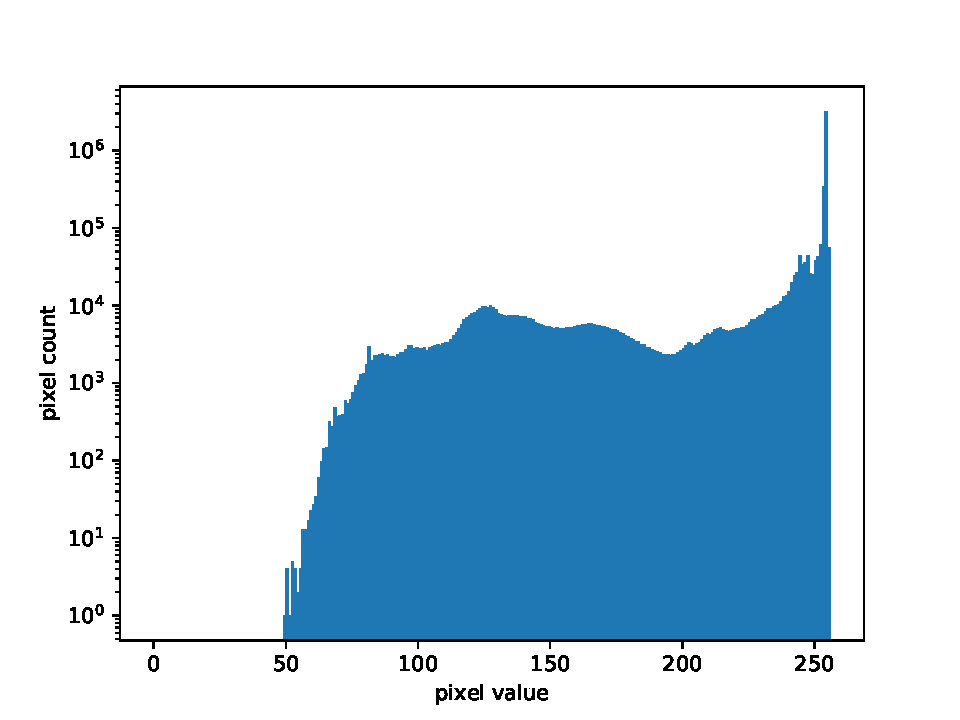
\includegraphics[width=7.95cm, keepaspectratio]{img/algos/tire_unwrapping-histogram_effect-hist_a.pdf}
            \caption{Hist. of Fig. \ref{fig:tire_unwrapping-equalization-effect}a}
            \label{fig:tire_unwrapping-hist_of_equalization_effect_a}
    \end{minipage}\hfill
\end{figure}

\begin{figure}
    \centering
    \begin{minipage}[c]{0.50\linewidth}
        \centering
        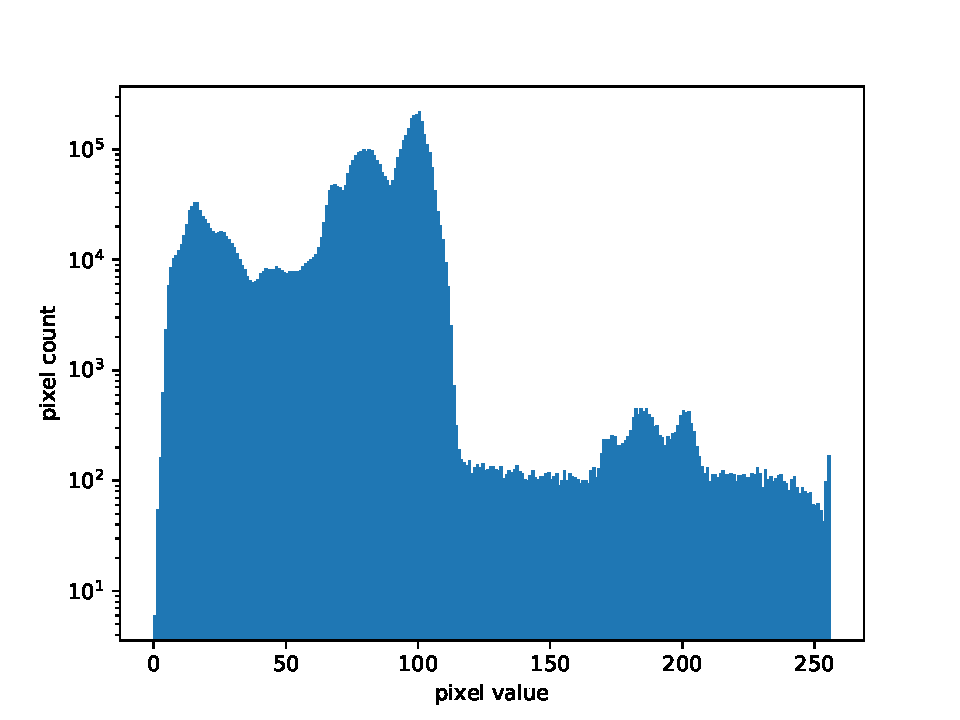
\includegraphics[width=7.95cm, keepaspectratio]{img/algos/tire_unwrapping-histogram_effect-hist_b.pdf}
        \caption{Hist. of Fig. \ref{fig:tire_unwrapping-equalization-effect}b}
        \label{fig:tire_unwrapping-hist_of_equalization_effect_b}
    \end{minipage}\hfill
    \begin{minipage}[c]{0.50\linewidth}
        \centering
        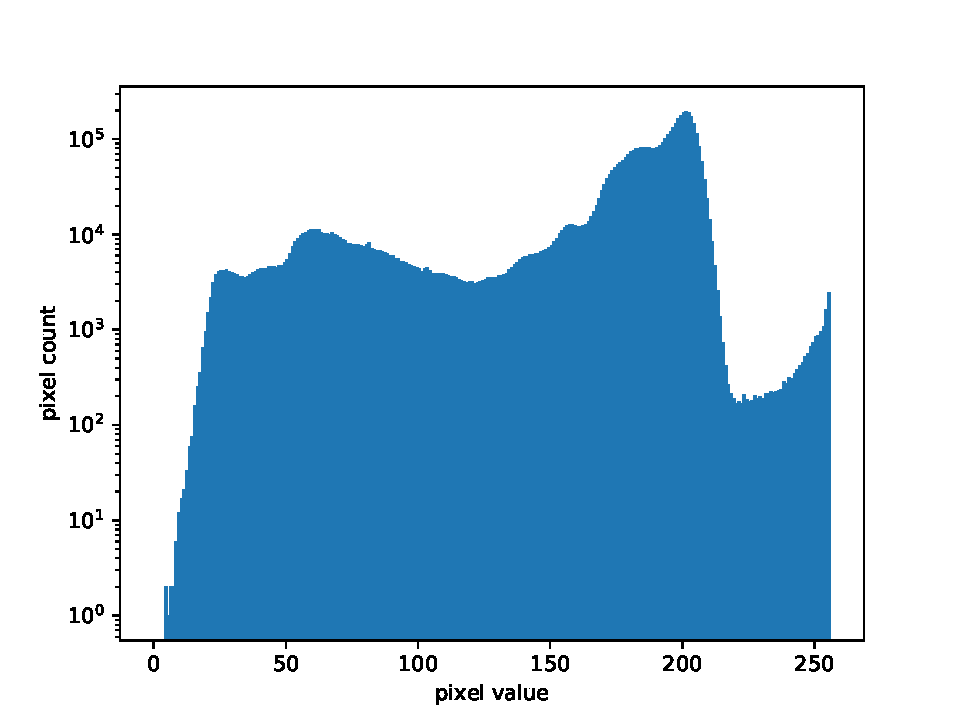
\includegraphics[width=7.95cm, keepaspectratio]{img/algos/tire_unwrapping-histogram_effect-hist_c.pdf}
        \caption{Hist. of Fig. \ref{fig:tire_unwrapping-equalization-effect}c}
        \label{fig:tire_unwrapping-hist_of_equalization_effect_c}
    \end{minipage}\hfill
\end{figure}

A deviation from this standard equalization is Adaptive Histogram Equalization (AHE) that is not applied on the entire image and just on a small portion of it. When calculating the new value for a pixel, only a neighborhood around it is taken into consideration. Thus method while useful in bringing more contrast in to an image that has lighter and darker regions, it also increases the noise in the image. To counteract this, Contrast Limited AHE (CLAHE) was created. The addition is that it has a clipping upper limit and redistributes the pixels that appear too often in the image into another ranges.

\paragraph*{Algorithm:}\mbox{}\par

\begin{algorithm}
    \caption{CLAHE}\label{alg:CLAHE}
    \begin{algorithmic}[1]
        \Require $img$ be a $X\times X$ matrix; $cl \in [0, 1]$; $k$

        \Ensure $k \mid X$

        \State $S \gets $ ($img$ split into $k\times k$ cells)\label{line:CLAHE:split}

        \For {$s$ in $S$}
            \State $H_s \gets histogram(s)$
            \State $H_{res}, N_{remain} \gets clip(H_s, cl)$
            % \State $N_{avg} \gets (k \times k) \div N_{gray}$
            % \State $N_{CL} \gets N_{clip} \times N_{avg}$
            % \State $N_{\Sigma\_clip} \gets \sum_{i=0}^{N_{gray}} max(0, H_s[i] - N_{CL})$
            % \State $N_{avg\_gray} \gets N_{\Sigma\_clip} \div N_{gray}$
            % \State $N_{remain} \gets N_{\Sigma\_clip}$
            % \For {$i=0:+1:N_{gray}$}
            %     \If {$H_s[i] > N_{CL}$}
            %         \State $H_{res}[i] \gets N_{CL}$
            %     \ElsIf {($H_s[i] + N_{avg\_gray}) > N_{CL}$}
            %         \State $N_{remain} \gets N_{remain} - (N_{CL} - H_s[i])$
            %         \State $H_{res}[i] \gets N_{CL}$
            %     \Else
            %         \State $N_{remain} \gets N_{remain} - N_{avg\_gray}$
            %         \State $H_{res}[i] \gets H_s[i] + N_{CL}$
            %     \EndIf
            % \EndFor

            \State $H_{res} \gets redistribute(H_{res}, N_{remain})$\label{line:CLAHE:redistribute}
            % \While {$N_{remain} > 0$}
            %     \State $step \gets N_{gray} \div N_{remain}$
            %     \For {$i=0:step:N_{gray}$}
            %         \If{$H_{res}[i] < N_{CL}$}
            %             \State $H_{res}[i] \gets H_{res}[i] + 1$
            %             \State $N_{remain} \gets N_{remain} - 1$
            %         \EndIf
            %     \EndFor
            % \EndWhile

            \State $s \gets adjust\_cell(s, H_{res})$
        \EndFor

        \State $img \gets$ interpolate cells $S$

    \end{algorithmic}
\end{algorithm}

CLAHE is described in pseudo-code in Algorithm \ref{alg:CLAHE} in accordance to the implementation found in \cite{site:CLAHE_code} and the explanation in the paper \cite{article:CLAHE_explanation}.

On line \ref{line:CLAHE:split} we split the image in multiple cells of size $k$ by $k$ because CLAHE is an adaptive algorithm.
Then, for each of the cells we calculate their histogram to find out how many different pixel values they contain ($N_{gray}$). To perform the clipping, we need to calculate a few things:

$N_{avg} \gets (k \times k) \div N_{gray}$, that is the number of pixels in the cell divided by how many pixel values are present in the cell;

$N_{CL} \gets cl \times N_{avg}$, the clipping limit calculated based on input parameter $cl$;

$N_{\Sigma\_clip} \gets \sum_{i=0}^{N_{gray}} max(0, H_s[i] - N_{CL})$, is the number of pixels that need to be clipped, $H_s[i]$ is the pixel count for a certain pixel value;

$N_{avg\_gray} \gets N_{\Sigma\_clip} \div N_{gray}$, is how many pixels in average we will modify in addition to have a certain value.

Then, we iterate through all the pixel values in the histogram and create a new one. If the pixel count is $\geq$ than $N_{CL}$, we will clip that pixel value. Else, we will add to the pixel count $N_{avg\_gray}$ and if we exceed the clipping limit, we floor to it and take note of this in the form of $N_remain$. After this step, the histogram would look like in figure \ref{fig:CLAHE_hist}.

\begin{figure}
    \centering
    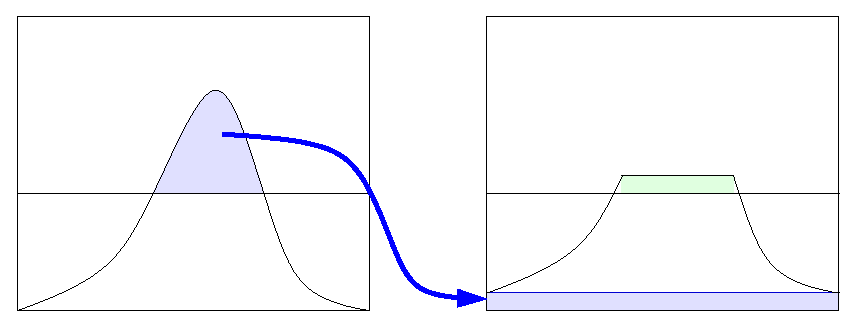
\includegraphics[width=0.4\columnwidth]{img/algos/Clahe-redistribution.eps}
    \caption{The histogram after first clipping, source: \cite{site:CLAHE_clipping_image}}
    \label{fig:CLAHE_hist}
\end{figure}

The limit we excede with will be redistributed after this on line \ref{line:CLAHE:redistribute}. Here, we go through the pixel values in the histogram again and at a simmilary random step we add one more pixel to the count that overflowed earlyer. The step is computed by the formula: $step \gets N_{gray} \div N_{remain}$.

Before starting to compute the next cell, we adjust the current one acoording to the new histogram we just computed: $H_{res}$.

After all the cels were modified and equalized, we can stisch them back together. But because we had a cell by cell approach to calculating the histogram, border pixels might have very different values. This is why an extra step of bilinear interpolation is performed on the border pizels of each of the cells.

\paragraph*{Results:}\mbox{}\par
If before the equalization the histogram of the image looked like Figure \ref{fig:tire_unwrapping-hist_of_uneq_img}, after the equalization it looks like Figure \ref{fig:tire_unwrapping-hist_of_eq_img}. It can be observed it is smoother and part of the pixels were brightened.

\begin{figure}
    \centering
    \begin{minipage}[c]{0.50\linewidth}
        \centering
        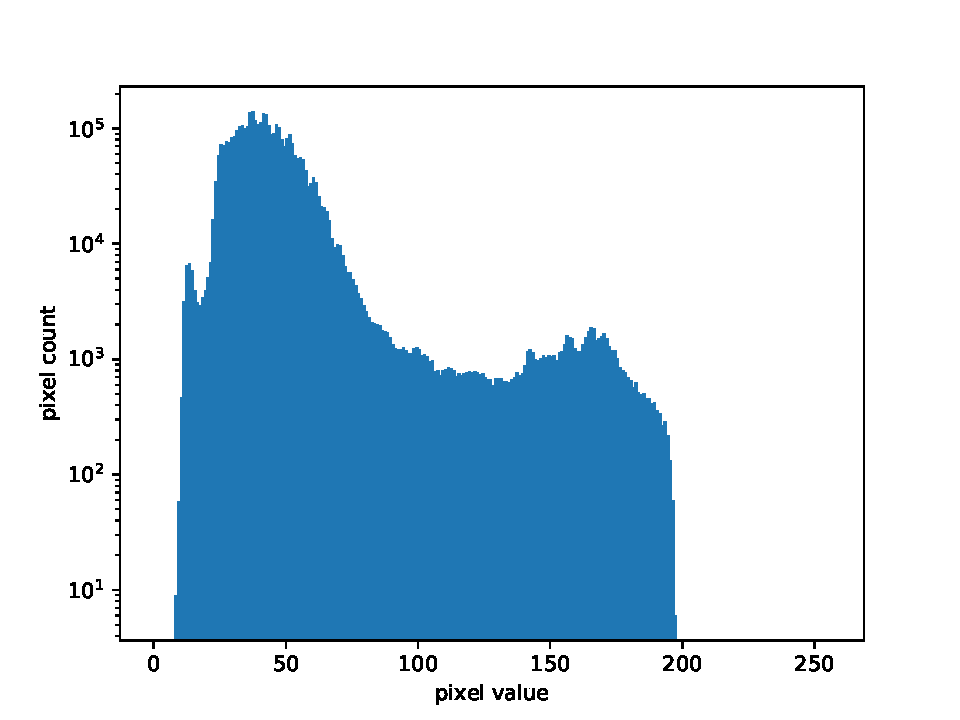
\includegraphics[width=7.95cm, keepaspectratio]{img/algos/tire_unwrapping-histogram_of_uneq_image.pdf}
        \caption{Histogram without equalization}
        \label{fig:tire_unwrapping-hist_of_uneq_img}
    \end{minipage}\hfill
    \begin{minipage}[c]{0.50\linewidth}
        \centering
        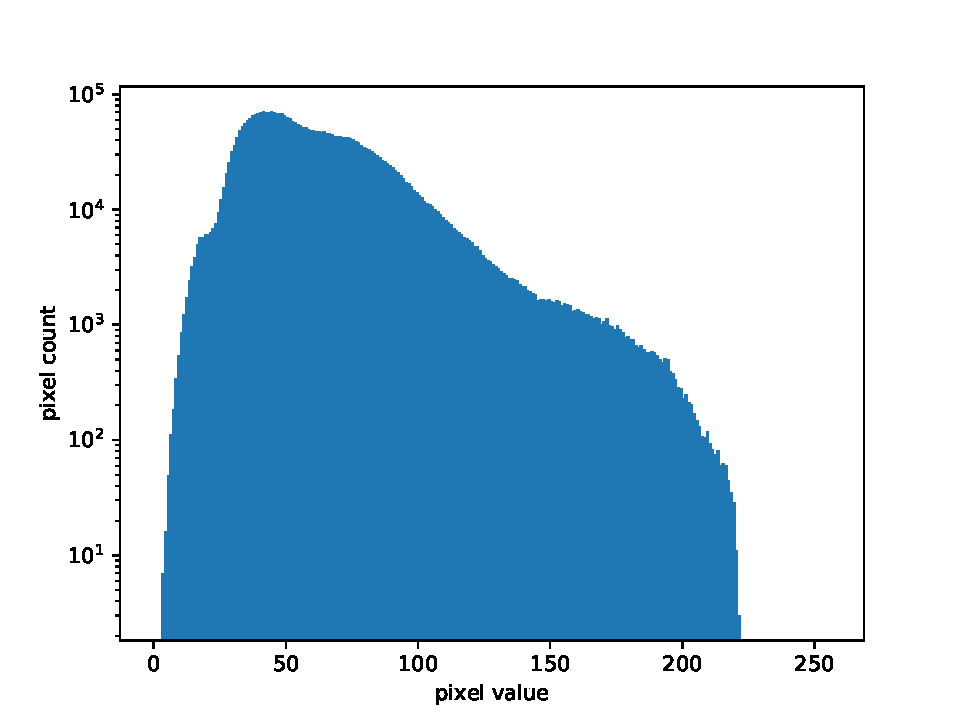
\includegraphics[width=7.95cm, keepaspectratio]{img/algos/tire_unwrapping-histogram_of_eq_image.pdf}
        \caption{Histogram with equalization}
        \label{fig:tire_unwrapping-hist_of_eq_img}
    \end{minipage}\hfill
\end{figure}

%%%%%%%%%%%%%%%%%%%%%%%%%%%%%%%%%%%%%%%%%%%%%%%%%%%%%%%%%%%%
%%% b) HOUGH CIRCLES TRANFORM                             %%%
%%%%%%%%%%%%%%%%%%%%%%%%%%%%%%%%%%%%%%%%%%%%%%%%%%%%%%%%%%%%

\subsubsection{Hough Circles Transform (HCT)}
\label{subsubsec:hough_circles_transform}

\paragraph*{Accomplishes:}\mbox{}\par
It detects circular shapes present in an image. The ones we are interested in are the outer and inner rims of the tire.

\paragraph*{Reasoning:}\mbox{}\par
The reasoning for why we want to detect the tire in the image is twofold. Firstly, the text searching part is a computational expensive one and we want to reduce the search space from the whole 3456 by 3456 pixels to usually a forth of that. The second reason is that the text is present in the image in a circular form, while the vast majority of optical character recognition (OCR) software is performing best on text that is aligned along one dimension only. So, by detecting the tire's circular shape in the image, we can transform the tire into its unwrapped version (that also has a smaller pixel count).

\paragraph*{Algorithm:}\mbox{}\par

\begin{algorithm}
    \caption{Hough Circles Transform}\label{alg:Hough_Circles}
    \begin{algorithmic}[1]
        \Require $img$; $r_{min}$; $r_{max}$; $dp$; $canny\_params$

        \State $blur \gets gaussian\_blur(img)$
        \State $gray \gets color2gray(blur)$
        \State $edges \gets canny(gray, canny\_params)$

        \For{$r=r_{min}:+1:r_{max}$}\label{line:Hough_Circles:for_r}
            \State $acc[i] \gets matrix(shape(img) \div dp)$
            \For{each pixel $p > 0$ in $edges$}\label{line:Hough_Circles:for_p}
                \State $acc[i] \gets accumulate(acc[i], p, r)$
            \EndFor
        \EndFor
    \State $center, radius \gets extract(acc)$\label{line:Hough_Circles:extract}
    \State \Return $(center, radius)$
    \end{algorithmic}
\end{algorithm}

Hough Circles Transform is particularization of the classical Hough Transform \cite{site:circular_hough_transform} and its scope is to extract features from images. The original algorithm is searching for a circle with a known radius, but as can be seen in Algorithm \ref{alg:Hough_Circles}, it can be generalized to an interval of radii.

The first 2 actions in the algorithm are to apply Gaussian Blur \cite{site:Gaussian_blur} (to remove the noise that follows a Gaussian distribution) and convert the color image into gray-scale.

Then it uses Canny Edge Detector \cite{site:Canny_edge_detection} to obtain a new image which contains only the outlines where the algorithm considered a boundary between 2 objects exists. An example can be seen in Figure \ref{fig:canny_output_tire}, where each white pixel represents an edge.

On line \ref{line:Hough_Circles:for_r}, it can be seen the $loop$ that will probe for the radius interval that was requested.

For each radius that the algorithm will probe, will create an accumulator matrix that is $dp$ times smaller than the original image. The purpose of this matrix will be explained shortly.

The central part of the algorithm is the for loop on line \ref{line:Hough_Circles:for_p}. It goes through all the pixels that resulted in being edges and finds their corresponding position in the smaller $acc[i]$ matrix. Then, all around that point in the accumulator matrix at distance $r$, it increments the corresponding cell. Four probed pixels (the white squares) of this can be seen in in Figure \ref{fig:Hough_circle_accumulator} where it can be seen that when circles overlap the value in that cell increases.

Such an accumulator is created for each probed radius and it will result in a 3D space. So, the last action of the algorithm (line \ref{line:Hough_Circles:extract}) is to search in this 3D space of accumulators and find the most incremented cell (the red dot in Figure \ref{fig:Hough_circle_accumulator}). That cell is considered the center of the circle and the radius is corresponding to the accumulator matrix it was found in.

\begin{figure}
    \centering
    \begin{minipage}[c]{0.33\linewidth}
        \centering
        \includegraphics[width=4.25cm, height=4.25cm]{img/algos/tire_unwrapping-Canny_wheel.jpg}
            \caption{Canny output}
            \label{fig:canny_output_tire}
    \end{minipage}\hfill
    \begin{minipage}[c]{0.33\linewidth}
        \centering
        \includegraphics[width=4.25cm, height=4.25cm]{img/algos/tire_unwrapping-HCT_acc.png}
            \caption{HCT accumulator}
            \label{fig:Hough_circle_accumulator}
    \end{minipage}\hfill
    \begin{minipage}[c]{0.33\linewidth}
        \centering
        \includegraphics[width=4.25cm, height=4.25cm]{img/algos/tire_unwrapping-detected_circles.jpg}
        \caption{HCT result}
        \label{fig:Hough-Circles-Transform_result}
    \end{minipage}\hfill
\end{figure}

\paragraph*{Results:}\mbox{}\par
Because tires have different dimensions and an outer and inner rim, I have to search for multiple circles in the image. So, I probed for multiple radii and the algorithm found multiple circles in the image, as can be seen in Figure \ref{fig:Hough-Circles-Transform_result}. This will be the input for the next step, where through a series of heuristics the circle count will be reduced to only the most concentric ones and hopefully only 2.

%%%%%%%%%%%%%%%%%%%%%%%%%%%%%%%%%%%%%%%%%%%%%%%%%%%%%%%%%%%%
%%% c) HEURISTICS                                        %%%
%%%%%%%%%%%%%%%%%%%%%%%%%%%%%%%%%%%%%%%%%%%%%%%%%%%%%%%%%%%%

\subsubsection{Heuristics}
\label{subsubsec:circ_det_heuristics}

\paragraph*{Accomplishes:}\mbox{}\par
Reduces the number of detected circles in the previous step (Figure \ref{fig:Hough-Circles-Transform_result}) and remains only with 2 concentric circles representing the tire's inner and outer rims (Figure \ref{fig:Hough_Circles_Transform-filtered_circles}). If his step fails to remain with only 2 circles, then the image is discarded.

\paragraph*{Reasoning:}\mbox{}\par
There are many types of tires in the wild with different shapes and sizes, so it was better in the previous step to detect more circles in the image than to look for only 2 circles. When looking only for 2 circles using the Hough Circular Transform, the car's wheel arc can be falsely detected as a circle or the wheel cap can have a pattern on it that would falsely trick the circle detection algorithm. Because of this reason, I preferred to detect many false positives and at this stage filter through them and remain with only the mot concentric circles that have at least a certain radius difference. Another possible problem would be that the tire is not a perfect circle because of the contact point with the ground or because when taking the image, the camera sensor was not in line with the wheel's axle.

\paragraph*{Algorithm:}\mbox{}\par
The first heuristic I apply is to reduce the circles that are very similar one to another. I start from the most prominent circle found by the previous step. If the conditions $dist(c_1, c_2) < 0.5 \times size(img)$ and $\Big|r_1 - r_2\Big| < 0.37 * size(img)$ are found true, that means the circles are probably the same one and I calculate a mean one. The mean is calculated by taking the average of the centers and the average of the radii. In checking other circles, thisone will be used. The values for the thresholds were found experimentally.

The second heuristic's goal is to create 2 concentric circles. At first I was taking the biggest and smallest circles and using the average of their center's coordinates to calculate a new center. This gave unsatisfactory results as the computed center would be quite far from the true one and in the unwrapping phase, it would not make the tire a continuous horizontal strip. The improvement I ended up finding was that the smaller radius circle would have the center closer to the wheel's true center, so it would be better to use the inner circle as the base rather than to calculate a new center. The reason to why the smaller circle has a better center is that the inner circle usually represents the inner rim of the tire that is a perfect circle, while the outer rim is deformed at the contact point between the ground and the wheel. That deformity can trow off the center calculated at the previous step. If more than 2 circles are present, this step is skipped and the image will be discarded as we couldn't detect the inner and outer parts of the tire. An improvement that could be made is that if more circles are found, to select the ones that have the closest centers and a radius bigger than a certain value.

\paragraph*{Results:}\mbox{}\par
The resulted concentric circles that can be seen in Figure \ref{fig:Hough_Circles_Transform-filtered_circles} are an approximation of what the true circle might be, but it is close enough so that the tire can be unwrapped. The circle might not follow perfectly the rim of the tire because of the distortion of the wheel on the ground, or the distortion was introduced when taking the picture if the camera's sensor wasn't horizontal and in line with the wheel's axle. If we couldn't remain with 2 concentric circles at this step, the image is discarded. Otherwise, it is passed to the next step.

\begin{figure}
    \centering
    \includegraphics[width=4.25cm, height=4.25cm]{img/algos/tire_unwrapping-filtered_circles.jpg}
    \caption{Filtered Concentric Circles Detected}
    \label{fig:Hough_Circles_Transform-filtered_circles}
\end{figure}

%%%%%%%%%%%%%%%%%%%%%%%%%%%%%%%%%%%%%%%%%%%%%%%%%%%%%%%%%%%%%%%%%%%%%%%%%%%%%%%%%%%%%%%%%%%%%%%%%%%%%%%%%%%%%%%%%%%%%%%%
\subsection{Convert to Polar Coordinates}
\label{subsec:convert_to_polar}

\paragraph*{Accomplishes:}\mbox{}\par
This step unwraps the tire and outputs it as a continuous horizontal strip as can be seen in Figure \ref{fig:tire_unwrapping-unwrapped}. This can be done because we have detected the supposed center of the tire and its radius.

\paragraph*{Reasoning:}\mbox{}\par
The horizontal strip will help in text detection and recognition, as it is easier to work with text going in only one direction.

\paragraph*{Algorithm:}\mbox{}\par
A normal image representation is in the Cartesian domain. In this domain, a pixel is characterized as having 2 coordinates: $x$ and $y$ that we are familiar with. So a pixel is defined by 2 distances and the 2 distances have an unique pixel tied to them.
Another domain to represent images in, is the Polar domain. In this domain, a pixel is characterized also with 2 coordinates: $angle$ and $radius$. The entire image is constructed around a center point and if information in the Cartesian domain was arranged in as the height of the image is the $y$ and the width is the $x$, here they are the $angle$ and $radius$ respectively.

Because of this correlation, we can convert from one domain to another. We are interested now in converting from a Cartesian system into a Polar one as the tire has a circular shape. We can use the found circle center to make it the origin of the new Polar domain and start taking points from the image starting at the small radius until the big one. For each pixel in the image, now with the found circle's center as the image's one, we can find its new $x$ and $y$ coordinate and from them, we can calculate its representation as $angle$ and $radius$ using the following formulas.

$radius = \sqrt{x^2 + y^2}$

$angle = \arctan(y/x)$

There is a problem though. Closer we are to the new selected center, less points are present on the surrounding circle than on a bigger one. The resulting image after the Polar transformation will have as it's width the pixel count of the pixels that were on the most outer circle's perimeter. The points closer to the center must be stretched out in order to fill in the gaps and this is solved using interpolation. New computed pixels are used to fill in the gaps.

\paragraph*{Results:}\mbox{}\par
Multiple interpolation levels were used to observe if it affects in any way the output, but the letters on the tire are far away from the detected center around which the polar transform si applied that even a bilinear interpolation is good. Now, I have the unwrapped tire as a new image (Figure \ref{fig:tire_unwrapping-unwrapped}) and it is ready to be processed further in order to obtain the regions of text. It must be mentioned that some wheel centers are falsely recognized and after the polar transform an unusable image is generated, like can be seen in Figure \ref{fig:tire_unwrapping-unwrapped-failed}. These are found and removed manualy and are not used in the next stages.

\begin{figure}
    \centering
    \includegraphics[width=\linewidth, keepaspectratio]{img/algos/tire_unwrapping-unwrapped.jpg}
    \caption{Successfully Unwrapped tire}
    \label{fig:tire_unwrapping-unwrapped}
\end{figure}
\begin{figure}
    \centering
    \includegraphics[width=\linewidth, keepaspectratio]{img/algos/tire_unwrapping-unwrapped-failed.png}
    \caption{Failed unwrapping of tire}
    \label{fig:tire_unwrapping-unwrapped-failed}
\end{figure}

%%%%%%%%%%%%%%%%%%%%%%%%%%%%%%%%%%%%%%%%%%%%%%%%%%%%%%%%%%%%%%%%%%%%%%%%%%%%%%%%%%%%%%%%%%%%%%%%%%%%%%%%%%%%%%%%%%%%%%%%
%%%%%%%%%%%%%%%%%%%%%%%%%%%%%%%%%%%%%%%%%%%%%%%%%%%%%%%%%%%%%%%%%%%%%%%%%%%%%%%%%%%%%%%%%%%%%%%%%%%%%%%%%%%%%%%%%%%%%%%%
%%%%%%%%%%%%%%%%%%%%%%%%%%%%%%%%%%%%%%%%%%%%%%%%%%%%%%%%%%%%%%%%%%%%%%%%%%%%%%%%%%%%%%%%%%%%%%%%%%%%%%%%%%%%%%%%%%%%%%%%
\section{Text Detection (Stage 2)}\label{sec:text-detection}
Now that the initial image was processed and just the tire region was kept and unwrapped to have a rectangular form with the text spanning from left to right, the text detection phase can begin. The goal now is to obtain a bitmap of the rectangular tire with regions where text is present. This phase is useful because it will further reduce the space where we have to perform text recognition, and because the goal is to reduce, false-positives are permitted in an acceptable limit. If we can reduce the image search space by at least 80\%, this stage is considered successful and the text recognition can begin. Otherwise the image is discarded.

%%%%%%%%%%%%%%%%%%%%%%%%%%%%%%%%%%%%%%%%%%%%%%%%%%%%%%%%%%%%%%%%%%%%%%%%%%%%%%%%%%%%%%%%%%%%%%%%%%%%%%%%%%%%%%%%%%%%%%%%
\subsection{Segmentation}
\label{subsec:segmentation}

\paragraph*{Accomplishes:}\mbox{}\par
Splits the image in smaller cells in order to perform operations on each one of them. These cells are overlapped a certain percentage to be able to vote on them regions of interest.

\paragraph*{Reasoning:}\mbox{}\par
While searching a way to obtain the text region in an image, frequency filtering proved useful and not needing parameter tuning. The less ideal part is that the last step is OTSU thresholding that is a global algorithm. While not performing useful if we were to process the entire image at the same time, it proved very helpful in binarizing smaller areas of the big image. So, I decided to split the original image in overlapping cells.

The cells overlap because in the end a voting process is employed to remove regions that were considered text in just a few of the segments.

\paragraph*{Algorithm:}\mbox{}\par
I need to calculate the corners of cells that have a certain overlap between them. This overlap is present on the $x$ and $y$ axes. Firstly, I calculate the number of cells that will be needed on each of the axes with the formula:
\[N = \frac{L - o}{no}\]
where $L$ is the number of pixels, $o$ is the size of the overlap region and $no$ is the region of a cell that is not overlapped.

\paragraph*{Results:}\mbox{}\par
Now the big picture was split in multiple smaller overlapping cells (Figure \ref{fig:text_detection-segment}) that will be further processed individually.

\begin{figure}
    \centering
    \includegraphics[height=6cm, keepaspectratio]{img/algos/text_detection-img_to_filter.jpg}
    \caption{Segment}
    \label{fig:text_detection-segment}
\end{figure}

%%%%%%%%%%%%%%%%%%%%%%%%%%%%%%%%%%%%%%%%%%%%%%%%%%%%%%%%%%%%%%%%%%%%%%%%%%%%%%%%%%%%%%%%%%%%%%%%%%%%%%%%%%%%%%%%%%%%%%%%
\subsection{Segment Binarization}

%%%%%%%%%%%%%%%%%%%%%%%%%%%%%%%%%%%%%%%%%%%%%%%%%%%%%%%%%%%%
%%% a) Frequency Filtering                               %%%
%%%%%%%%%%%%%%%%%%%%%%%%%%%%%%%%%%%%%%%%%%%%%%%%%%%%%%%%%%%%
\subsubsection{Image Frequency Filtering}
\label{subsubsec:frequency-filtering}

\paragraph*{Accomplishes:}\mbox{}\par
This is a band-pass filter applied to the frequency domain of the segment. The remaining frequencies will consist of letter shapes (the tire-markings) and some artifacts.

\paragraph*{Reasoning:}\mbox{}\par
Because the background of the tire is fairly uniform in blackness and noise, these can be considered low frequency color variations and high frequency noise respectively. By eliminating certain bands from the frequency domain of the image, we are left with the letter shapes that could be processed further to enhance them and filter out any artifacts that remained.

\paragraph*{Algorithm:}\mbox{}\par

\begin{algorithm}
    \caption{Band-pass Filtering}\label{alg:frequency-filtering}
    \begin{algorithmic}[1]
        \Require $img$

        \State $f\_rep \gets FFT(img)$
        \State $f\_rep \gets bandpass\_filter(f\_rep, low, high)$
        \State $img \gets IFFT(f\_rep)$

    \end{algorithmic}
\end{algorithm}

\begin{figure}
    \centering
    \includegraphics[height=0.2\linewidth]{img/algos/image-freq-domain-example.png}
    \caption{Frequency domain representation}
    \label{fig:example-img-freq-domain}
\end{figure}

Any analog signal is composed from multiple signals of different frequencies. These frequencies could be extracted using Fourier Transform \cite{book:fourier_transform} or reconstruct the signal using its inverse. Because it is a computationally expensive algorithm, in practice Fast Fourier Transform \cite{book:fourier_transform} is used because it usually gives acceptable results.

This step can be described by Algorithm \ref{alg:frequency-filtering}. But firstly, it must be made clear what passing an image into the frequency domain means. The easiest is to take a one dimensional example (a line) and then generalize for a two dimensional case (an image).

On the line, each pixel value could be considered to represent the amplitude of a signal. The signal progresses in time to one direction of the line. This signal can be decomposed in its core frequencies, to the left the low ones and the high ones to the right. The same thinking could be also applied to a 2D image, just that we get a 2D frequency image with real and imaginary components. For example, Figure \ref{fig:example-img-freq-domain} represents what happens if we have only a frequency present, what the resulting image would look like. The distance from the corner represents the frequency, while the position of the dot is the angle the bands will appear after applying the Inverse Fourier Transform.

To be easier to visualize the frequencies, the image is usually shifted so that the 0 frequency is in the middle of the image rather than in the corners like in Figure \ref{fig:text_detection-freq_domain_original}. This is useful also because it makes it easier to apply a band-pass filter. To apply this, we just have to blackout the middle of the image and the outer parts. In the end we are left with a disk shaped frequency representation of the image (Figure \ref{fig:text_detection-freq_domain_filtered}). Experimentally I got usable results by keeping a disk with the small radius 14\% and the big radius 36\% of the found frequencies in the image.

After applying the Inverse Fast Fourier Transform, we can observe that the low (the background) and the high (the noise) frequencies were removed. I successfully removed the background and the noise and still remained with the general letter outline in the image as can be seen in Figure \ref{fig:text_detection-bandpassed_segment} and \ref{fig:text_detection-bandpassed_segment-zoomed}.

The huge benefit of this method is that it can be applied to more images using the same band-pass filter, without changing the cutoffs.

\begin{figure}
    \centering
    \begin{minipage}[c]{0.5\linewidth}
        \centering
        \includegraphics[height=6cm, keepaspectratio]{img/algos/text_detection-freq_domain-original.jpg}
        \caption{Frequency domain of Figure \ref{fig:text_detection-segment}}
        \label{fig:text_detection-freq_domain_original}
    \end{minipage}\hfill
    \begin{minipage}[c]{0.5\linewidth}
        \centering
        \includegraphics[height=6cm, keepaspectratio]{img/algos/text_detection-freq_domain-bandpassed.jpg}
        \caption{Filtered frequency domain of Figure \ref{fig:text_detection-segment}}
        \label{fig:text_detection-freq_domain_filtered}
    \end{minipage}\hfill
\end{figure}

\begin{figure}
    \centering
    \begin{minipage}[c]{0.37\linewidth}
        \centering
        \includegraphics[height=5.9cm, keepaspectratio]{img/algos/text_detection-bandpassed_img.jpg}
        \caption{Filtered segment \ref{fig:text_detection-segment}}
        \label{fig:text_detection-bandpassed_segment}
    \end{minipage}\hfill
    \begin{minipage}[c]{0.63\linewidth}
        \centering
        \includegraphics[width=9.6cm, keepaspectratio]{img/algos/text_detection-bandpassed_img-zoomed.jpg}
        \caption{Zoom on text in filtered segment \ref{fig:text_detection-bandpassed_segment}}
        \label{fig:text_detection-bandpassed_segment-zoomed}
    \end{minipage}\hfill
\end{figure}

\paragraph*{Results:}\mbox{}\par
Outputs an image like in Figure \ref{fig:text_detection-bandpassed_segment}, where letter shapes could be observed. There are also artifacts remaining that will be dealt with at a later stage.

%%%%%%%%%%%%%%%%%%%%%%%%%%%%%%%%%%%%%%%%%%%%%%%%%%%%%%%%%%%%
%%% b) Morphological Operation                           %%%
%%%%%%%%%%%%%%%%%%%%%%%%%%%%%%%%%%%%%%%%%%%%%%%%%%%%%%%%%%%%
\subsubsection{Black Hat Morphological Operation}
\label{subsubsec:bh-morpho-op}

\paragraph*{Accomplishes:}\mbox{}\par
Enhances the darker regions representing the letter contours that are surrounded by brighter regions.

\paragraph*{Reasoning:}\mbox{}\par
It can be seen that in the resulted image at the previous step (Figure \ref{fig:text_detection-bandpassed_segment}), the letters have an outline in dark pixels surrounded by bright regions. It can be more clearly seen in Figure \ref{fig:text_detection-bandpassed_segment-zoomed}. By extracting this outline of the letters, we will be able to have the letters more prominent in the image than other features.

\paragraph*{Algorithm:}\mbox{}\par
A morphological operation is based on mathematical morphology \cite{article:mathematical-morphology}. The main components to it are an object $A$ (our image) and a structuring element $B$. Normally, these operations are applied on binary images but variations exist that let them to be used also on gray-scale ones. Firstly, a path must be created for our structuring element ($B$) to traverse the edge of the object ($A$). This path if formally defined as a function that maps points from our image to a real line.
\[f:E \rightarrow R\]
The Black Hat Morphological operation is defined mathematically as:
\[T_b(f) = f \bullet b - f\]
where $b$ is a structuring element and $\bullet$ means the closing operation that is defined as a dilation followed by an erosion of a set $A$ by a structuring element $B$:
\[A \bullet B = (A \oplus B) \ominus B\]

\paragraph*{Results:}\mbox{}\par
The result of this step can be seen in Figure \ref{fig:text_detection-blackhat_on_bandpassed_segment}. The figure has the brightness increased for viewing, but even if it's a darker image, it would not be a problem for a thresholding algorithm that can select his own threshold. This is why, in the next step we apply OTSU thresholding.

\begin{figure}
    \centering
    \includegraphics[width=8cm, keepaspectratio]{img/algos/text_detection-blackhat_on_bandpassed.jpg}
    \caption{Blackhat applied on Figure \ref{fig:text_detection-bandpassed_segment}}
    \label{fig:text_detection-blackhat_on_bandpassed_segment}
\end{figure}

%%%%%%%%%%%%%%%%%%%%%%%%%%%%%%%%%%%%%%%%%%%%%%%%%%%%%%%%%%%%
%%% c) OTSU Thresholding                                 %%%
%%%%%%%%%%%%%%%%%%%%%%%%%%%%%%%%%%%%%%%%%%%%%%%%%%%%%%%%%%%%
\subsubsection{OTSU Thresholding}
\label{subsubsec:OTSU-binarization}

\paragraph*{Accomplishes:}\mbox{}\par
Computes automatically a threshold for the image and applies it, outputting a binary image. Because of the processing previously done, the output consists of tire-markings and some artifacts.

\paragraph*{Reasoning:}\mbox{}\par
When trying different methods to make the regions of interest (the tire-markings) remain in the image and remove the parts I am not interested in, OTSU Thresholding happened to do just that. Before the voting could begin, I anyway would have had to binarize the image so this is even more helpful. The fact that OTSU computes automatically its threshold is also very helpful as it prevents the need to experimentally fine tune the algorithm and perform overfitting. The output would have some artifacts that I removed as much as possible through a set of heuristics later.

\paragraph*{Algorithm:}\mbox{}\par
The novalty in the OTSU Thresholding (Algorithm \ref{alg:OTSU-thresholding}) is that it computes the threshold by minimizing the intra-class variance (the variance between the white and black pixels that would result).

For each possible threshold value computes the binary image. After which the algorithm computes on the respective image the variance in white and black pixels and returns the weighted variance of the two. This can be seen on line \ref{line:OTSU:variance-calculation} of the algorithm. We store the resulting image with the threshold and the weighted variance in 2 vectors ($I$ and $WV$) that are self incrementing.

As a last step (line \ref{line:OTSU:threshold-selection}) we select the threshold that minimizes the weighted variance and retuns the corresponding computed binary image with its corresponding threshold.

\begin{algorithm}
    \caption{OTSU Thresholding}\label{alg:OTSU-thresholding}
    \begin{algorithmic}[1]
        \Require $img$

        \For{$t$ in possible thresholds}
            \State $img_{bin} \gets threshold(img, t)$
            \State $I[i] \gets (img_{bin}, t)$
            \State $WV[i] \gets weighted_varianve(img_{bin})$\label{line:OTSU:variance-calculation}
        \EndFor
        \State $it \gets pos\_of\_min(WV)$\label{line:OTSU:threshold-selection}
        \State \Return $I[it]$
    \end{algorithmic}
\end{algorithm}

\paragraph*{Results:}\mbox{}\par
It can be seen in Figure \ref{fig:text_detection-OTSU_on_blackhat} that the letters or text remains almost as a connected component while the artifacts span across the entire segment or are small dots. This is very helpful as we can filter for the components that have a certain size and shape.

\begin{figure}
    \centering
    \includegraphics[width=8cm, keepaspectratio]{img/algos/text_detection-OTSU_on_blackhat.jpg}
    \caption{Supposed text areas (OTSU applied on Figure \ref{fig:text_detection-blackhat_on_bandpassed_segment})}
    \label{fig:text_detection-OTSU_on_blackhat}
\end{figure}

%%%%%%%%%%%%%%%%%%%%%%%%%%%%%%%%%%%%%%%%%%%%%%%%%%%%%%%%%%%%%%%%%%%%%%%%%%%%%%%%%%%%%%%%%%%%%%%%%%%%%%%%%%%%%%%%%%%%%%%%
\subsection{Filtering Artifacts}

\paragraph*{Accomplishes:}\mbox{}\par
The artifacts that can be seen in Figure \ref{fig:text_detection-OTSU_on_blackhat} are removed as much as possible, while retaining the letters' shapes in the binary map. This process is a combination of heuristics and morphological operations.

\paragraph*{Reasoning:}\mbox{}\par
Because the output of this step will be used in voting the regions of interest the text recognition will take place on, we would like to discard as many artifacts as possible. A big majority of them can be identified and removed because of their shape and size. The regions of text we are interested in are elongated and not very tall, while the letters have a common supple shape.

\paragraph*{Algorithm:}\mbox{}\par

\begin{algorithm}
    \caption{Filtering Artifacts}\label{alg:filtering-artifacts}
    \begin{algorithmic}[1]
        \Require $img$

        \State $img \gets dilate(img, se, 1)$
        \State $CCs \gets contours(img)$\label{alg:filtering-artifacts:contours-1}
        \State $img \gets filter(img, CCs, heu_1)$\label{alg:filtering-artifacts:filter-1}
        \State $img \gets dilate(img, se, 4)$
        \State $CCs \gets contours(img)$
        \State $img \gets filter(img, CCs, heu_2)$\label{alg:filtering-artifacts:filter-2}

        \State \Return $img$
    \end{algorithmic}
\end{algorithm}

The pseudo-code for the filtering process can be seen in Algorithm \ref{alg:filtering-artifacts}.

It starts off with a dilation, which is a morphological operation \cite{article:mathematical-morphology} which results in the thickening of the white connected components. It can be described mathematically as:

\[A \oplus B = \{z \in E | (B^s)_z \cap A \neq \emptyset \} \]
where $A$ is our image with sets in it, $B$ is a structuring element that is applied across the entirety of $A$ and $B^s$ is the symmetric of $B$. This is used in order to unite any artifacts and letter parts that might be disconnected because of the initial lighting conditions. For now I apply a single iteration.

The operation on line \ref{alg:filtering-artifacts:contours-1} looks in the image and finds all the connected components ($CCs$).

Then on line \ref{alg:filtering-artifacts:filter-1} we apply the first series of heuristics. These were determined experimentally and through the observation of the sizes of letters. On each component, a bounding box is placed. Any of the following rules ($heu_1$\label{filtering:heuristics-1}) would force the component to be discarded: $h < 10p \;|\; w < 10p$ (even if this was a letter, it would be too small to be recognizable), $h/w > 1.5 \;|\; h/w < 0.33$ or $h > 0.33*h_{seg} \;\&\; w > 0.66*w_{seg}$. ($h$ - height of the component, $w$ - width of the component, $h_{seg}$ - height of the segment, $w_{seg}$ - width of the segment).

After this first series of filtering noise, I've decided to apply again dilation operation but for 4 iterations in order to thicken up the remaining sets. I do not want necessarily to close the spaces between them, as I would have chosen to use the closing morphological operation if I wanted that.

I search again for the connected components ($CCs$) in the image as they might have changed quite drastically from the last time.

And now, as a last step (line \ref{alg:filtering-artifacts:filter-2}), I apply another filtration with other rules. In my experiments, I observed that some more artifacts could be eliminated at this step so I chose to do just that. The rules for removing these artifacts ($heu_2$\label{filtering:heuristics-2}) are:  $h < 26p \;|\; w < 10p$ (even if this was a letter, it would be too small to be recognizable), $h/w > 1.5 \;|\; h/w < 0.33$ or $h > 0.33*h_{seg} \;\&\; w > 0.66*w_{seg}$. Practically, almost the same rules as in the first round of filtration, just that now the height of the component must be bigger as we have applied dilation a few times already.

\paragraph*{Results:}\mbox{}\par
Even if the filtering process gives some false negatives and lets some artifacts to pass, it would be way worse to have false negatives and start removing from the tire-markings themselves. I am satisfied with the current state of the filter because as can be seen in Figure \ref{fig:text_detection-bitmap_segment} I could eliminate the vast majority of the artifacts present in Figure \ref{fig:text_detection-OTSU_on_blackhat}. This bitmap will be used for voting in the accumulator that has the same size with the unwrapped image.

Finding connected components is a quite expensive operation, so further improvement could be done on this step in order to reduce the number of searches for connected components to speed up the pipeline.

\begin{figure}
    \centering
    \includegraphics[width=6cm, keepaspectratio]{img/algos/text_detection-bitmap_segment.jpg}
    \caption{Resulted binary image with supposed text areas after artifact filtering}
    \label{fig:text_detection-bitmap_segment}
\end{figure}

%%%%%%%%%%%%%%%%%%%%%%%%%%%%%%%%%%%%%%%%%%%%%%%%%%%%%%%%%%%%%%%%%%%%%%%%%%%%%%%%%%%%%%%%%%%%%%%%%%%%%%%%%%%%%%%%%%%%%%%%
\subsection{Voting}

Now that the segment was processed (revealed the zone where text is present and removed as much as possible of the artifacts present in the image), the white zones that remained will have their corresponding place in the accumulator matrix (that is the same size with the unwrapped image) increased by one. This is the action that I called voting. Because of the overlap between segments this voting step can be used to further reduce the number of false positive regions of interest.

After all the segments were processed, it results a voting map like the one in Figure \ref{fig:text_detection-voting_map} (it was enhanced to be more visible), where the brighter the region, the more votes it got. But this voting accumulator can be further processed in order to reduce the zones that will remain as regions of interest for the text recognition part of the pipeline.

The filtration could be described by the pseudo-code in Algorithm \ref{alg:voting-filtering}. I start off with a threshold operation, where I discard any region that did not get at least 3 votes. This step is done to reduce the artifacts that appeared only in some segments. The thresholding operation also makes the pixels that passed the check to have the maximum value, resulting in the accumulator becoming a binary image.

\begin{algorithm}
    \caption{Cleaning Accumulator Matrix}\label{alg:voting-filtering}
    \begin{algorithmic}[1]
        \Require $acc$

        \State $acc \gets threshold(acc, 3)$
        \State $CCs \gets contours(acc)$\label{alg:voting-filtering:contours-1}
        \State $acc \gets filter(acc, CCs, heu_3)$\label{alg:voting-filtering:filter-1}
        \State $acc \gets dilate(acc, se, 4)$
        \State $CCs \gets contours(acc)$
        \State $acc \gets filter(acc, CCs, heu_4)$

        \State \Return $acc$
    \end{algorithmic}
\end{algorithm}

Then, on line \ref{alg:voting-filtering:filter-1} I am filtering through the connected components found in the accumulator matrix (the operation on line \ref{alg:voting-filtering:contours-1}). The component is discarded if its bounding box has $h < 40p \;|\; w < 10p$ ($heu_3$\label{filtering:heuristics-3}) as it would be too small to be even a letter. At this step the height limit was increased compared to heuristic \hyperref[filtering:heuristics-2]{$hre_2$} because the components that are voted by multiple segments tend to thicken up. This might be because of the frequency filtering leaves different aspects of a feature (tire-marking or artifact) visible as it is very dependable on the content of the segment.

On the filtered accumulator matrix, 4 iterations of the morphological operation dilation were applied to connect the letters. Other artifacts that are still present would not connect with anything else if they are far away enough from other connected components.

Now, on the newly diluted accumulator matrix and the new connected components, we apply another filtration using the heuristics $heu_4$\label{filtering:heuristics-4} that consist of: heuristic \hyperref[filtering:heuristics-3]{$hre_3$}, $h > 200p$ (the text region is too tall so it is a region that we are not interested in) or $h > 100p \;\&\; h/w > 0.85$ (a region too tall that doesn't have a prominent enough shape).

The result of this step is a bitmap (Figure \ref{fig:text_detection-binarymap}) that when applied over the wrapped tire shows regions of text (Figure \ref{fig:text-regions-on-unwrapped-tire}). This bitmap will be used in the text recognition stage to indicate the regions of interest in the image and reduce the space on wich the algorithm will run on.

\begin{figure}
    \centering
    \includegraphics[width=15.9cm, keepaspectratio]{img/algos/text_detection-voting_map.png}
    \caption{Voting map}
    \label{fig:text_detection-voting_map}
\end{figure}

\begin{figure}
    \centering
    \includegraphics[width=\linewidth, keepaspectratio]{img/algos/text_detection-binarymap1.png}
    \caption{Binary map with text regions}
    \label{fig:text_detection-binarymap}
\end{figure}

\begin{figure}
    \centering
    \includegraphics[width=15.9cm, keepaspectratio]{img/algos/text_detection-bounding_boxes_on_detected_text.png}
    \caption{Text Regions on Unwrapped Tire}
    \label{fig:text-regions-on-unwrapped-tire}
\end{figure}

%%%%%%%%%%%%%%%%%%%%%%%%%%%%%%%%%%%%%%%%%%%%%%%%%%%%%%%%%%%%%%%%%%%%%%%%%%%%%%%%%%%%%%%%%%%%%%%%%%%%%%%%%%%%%%%%%%%%%%%%
%%%%%%%%%%%%%%%%%%%%%%%%%%%%%%%%%%%%%%%%%%%%%%%%%%%%%%%%%%%%%%%%%%%%%%%%%%%%%%%%%%%%%%%%%%%%%%%%%%%%%%%%%%%%%%%%%%%%%%%%
%%%%%%%%%%%%%%%%%%%%%%%%%%%%%%%%%%%%%%%%%%%%%%%%%%%%%%%%%%%%%%%%%%%%%%%%%%%%%%%%%%%%%%%%%%%%%%%%%%%%%%%%%%%%%%%%%%%%%%%%
\section{Text Recognition (Stage 3)}\label{sec:text-recognition}

\paragraph*{Accomplishes:}\mbox{}\par

Now that we have reduced our unwrapped image to a few regions of interest, we can use an OCR to start extracting the text. This will be the output of our system and it will define our performance. The quality of the input images is also an important factor because during the evaluation of the system I observed that blurry and darker images (like Figure \ref{fig:text_recognition-blurry_image}) -- which translates in a lower contrast in the image -- have the text not recognized at all.

\paragraph*{Reasoning:}\mbox{}\par

It could be considered that the reason is stated in the \hyperref[sec:motivation]{Motivation} section of this work, but to reiterate, we want to extract the serial DOT code and the E-mark certification in order to almost uniquely identify a tire. I chose to use an OCR for this stage because they are the most common approach to text recognition and the availability of ready made solutions only increased in the past years \cite{site:OCR_comparison}. There is also a wide variety to the OCR solutions that are offered as services, accessible through APIs.

\paragraph*{Algorithm:}\mbox{}\par
The OCR I used is a service from Microsoft Cognitive Solutions \cite{site:Microsoft_Cognitive_Services} and it uses "deep-learning-based models and works with text on a variety of surfaces and backgrounds" (source: \cite{site:Microsoft_Cognitive_Services-Explained}). So, it is not specially tailored to our case (tire images). This is a good thing as it provides versatility at the expense of performance and openness of the system.

The Read API (that is the OCR's name) \cite{site:Microsoft_Cognitive_Services-Read_API-OCR} is accessed through API calls to a configured endpoint. For each region of interest extracted in the Text Detection \ref{sec:text-detection} section, a request is sent to the endpoint which returns its guess on the text in the image. While not being able to perform all the processing on only one local machine (as we had to rely on the computation power and OCR solution hosted on a remote server), the impact this has on performance is reduced because we submit only the regions of interest (which have a smaller size than the original unwrapped tire image).

\begin{figure}
    \centering
    \includegraphics[width=15.9cm, keepaspectratio]{img/algos/text_recognition-blurry_image.png}
    \caption{Blurry and lower contrast image}
    \label{fig:text_recognition-blurry_image}
\end{figure}

\paragraph*{Results:}\mbox{}\par
The results from this stage are in the form of annotations that are coupled with the original detected region of interest. The recognized text returned by the OCR will be categorized in the following categories: DOT serial code, E-Mark certification and miscellaneous.

% %%%%%%%%%%%%%%%%%%%%%%%%%%%%%%%%%%%%%%%%%%%%%%%%%%%%%%%%%%%%
% %%% x) TEMPLATE                                          %%%
% %%%%%%%%%%%%%%%%%%%%%%%%%%%%%%%%%%%%%%%%%%%%%%%%%%%%%%%%%%%%

% % TODO: remove
% \subsubsection{TEMPLATE}
% \label{subsubsec:TEMPLATE}

% \paragraph*{Accomplishes:}\mbox{}\par

% \paragraph*{Reasoning:}\mbox{}\par

% \paragraph*{Algorithm:}\mbox{}\par

% \paragraph*{Results:}\mbox{}\par
